\subsection{Question 1}
\subsubsection{Part A}

Method 1: \(LU\) factor \(A-sI\) for \(s=0\) and \(s=1\) and inspecting the number of negative values on the diagonal of \(U\).

Case 1: \(s=0\),

\begin{eqnarray}
  A_0 = 
  \begin{pmatrix}
    -1 & 1 & 0 \\
    1 & 1 & 1 \\
    0 & 1 & 2 \\
  \end{pmatrix}
\end{eqnarray}

\begin{eqnarray}
  L_0 =
  \begin{bmatrix}
    1 & 0 & 0 \\
    -1 & 1 & 0 \\
    0 & 0 & 1 \\
  \end{bmatrix}
  , U_0 =
  \begin{bmatrix}
    -1 & 1 & 0 \\
    0 & 2 & 1 \\
    0 & 0 & 1.5 \\
  \end{bmatrix}
  \\
  L_1 = 
  \begin{bmatrix}
    1 & 0 & 0 \\
    -1 & 1 & 0 \\
    0 & 0.5 & 1 \\
  \end{bmatrix}
  , U_1 = 
  \begin{bmatrix}
    -1 & 1 & 0 \\
    0 & 2 & 1 \\
    0 & 0 & 1.5 \\
  \end{bmatrix}
\end{eqnarray}

Therefore, when we inspect the diagonal of \(U_1\) we see that there is one negative value.
This means that there is one eigenvalue in \(A\) that is less than zero.

Case 2: \(s=1\),


\begin{eqnarray}
  A_1 = 
  \begin{pmatrix}
    -2 & 1 & 0 \\
    1 & 0 & 1 \\
    0 & 1 & 1 \\
  \end{pmatrix}
\end{eqnarray}

\begin{eqnarray}
  L_0 =
  \begin{bmatrix}
    1 & 0 & 0 \\
    -0.5 & 1 & 0 \\
    0 & 0 & 1 \\
  \end{bmatrix}
  , U_0 =
  \begin{bmatrix}
    -2 & 1 & 0 \\
    0 & 0.5 & 1 \\
    0 & 1 & 1 \\
  \end{bmatrix}
  \\
  L_1 = 
  \begin{bmatrix}
    1 & 0 & 0 \\
    -0.5 & 1 & 0 \\
    0 & 2 & 1 \\
  \end{bmatrix}
  , U_1 = 
  \begin{bmatrix}
    -2 & 1 & 0 \\
    0 & 0.5 & 1 \\
    0 & 0 & -1 \\
  \end{bmatrix}
\end{eqnarray}

Therefore, when we inspect the diagonal of \(U_1\) we see that there are two negative values.
This means that there are two eigenvalues in \(A\) that are less than one.
Utilizing the knowledge from both cases we have found that there is one eigenvalue in the range \([0,1]\).

\newpage
Method 2: Compute the number of sign changes in the sequence of main principal minors of \(A-sI\) for \(s=0\) and \(s=1\).

\lstinputlisting[caption=Matlab Commands,showstringspaces=false,language=Matlab]{../mpm.m}
\lstinputlisting[caption=Matlab Commands,showstringspaces=false,language=Matlab]{../q1_partA}

We see that in case 1 there is one sign change in the sequence of main principal minors and that in case 2 there are two sign changes in the sequence of main principal minors.
Therefore, as with method 1 we have shown there is a single eigenvalue in the range \([0,1]\).

\subsubsection{Part B}

The best estimate count of arithmetic operations for the two methods was 116 flops for method 1 and 36 flops for method 2.
Therefore, it would seem that method 2 is more efficient for tridiagonal matrices and it makes intuitive sense that this gap will become larger as the matrices grow in size ({\em i.e.,} method 2 will look better and better relative to method 1).

\newpage
\subsubsection{Part C}

The code below generates 100 symmetric tridiagonal matrices of size 50x50 and runs both Method 1 and Method 2 from part A.
\lstinputlisting[caption=Matlab Commands,showstringspaces=false,language=Matlab]{../q1_partC.m}
\lstinputlisting[caption=Matlab Commands,showstringspaces=false,language=Matlab]{../sign_changes.m}

The results of the code snippet above are presented below.
It is clear as stated in part B that Method 2 dominates Method 1 in terms of running speed.
This contrast grows as the size of the symmetric tridiagonal matrix grows.
\lstinputlisting[caption=Matlab Commands,showstringspaces=false,language=Matlab]{../q1_partC}

\newpage
\subsection{Question 2}
\subsubsection{Part A}

Since the Gerschgorin's disks are pairwise disjoint we know that each disk must contain one eigenvalue.
Therefore the cardinality of \(\sigma(A) = n\).
This means that the algebraic multiplicity \(m_a\) of each eigenvalue is \(m_a = 1\).
We know that the geometric multiplicity \(m_g\) follows the rule \(m_g \leq m_a\) for all eigenvalues of \(A\).
Therefore, since \(m_a = 1\) we can say that \(m_g = 1\). 

\subsubsection{Part B}

Leon is correct because as stated above \(m_g = m_a\) for eigenvalues of \(A\).


\subsubsection{Part C}

Nina is correct because there are \(n\) eigenvalues; one per disk.
If there was a complex eigenvalue it's complex conjugate would be an eigenvalue as well.
This would require two eigenvalues to be located in a single disk.
However this would contradict what we have shown in (a).
Therefore all eigenvalues of \(A\) are real.

\subsubsection{Part D}

Elvis is not correct.
The problem is that there can be two distinct eigenvalues in the real that have the same magnitude.
For example, suppose a matrix \(B\) as eigenvalues \(\lambda_{1} = 6, \lambda_{2} = -6\).
It is clear, \(|\lambda_{1}| = |\lambda_{2}|\).
In this case the power method will not converge because there is no dominant eigenvalue.

\newpage
\subsection{Question 3}

\lstinputlisting[caption=Matlab Commands,showstringspaces=false,language=Matlab]{../q3.m}
\newpage
\lstinputlisting[caption=Matlab Commands,showstringspaces=false,language=Matlab]{../q3_results}

There are two main issues or problems that may arise during this procedure.
The first is that the method simply will not converge (or at least converge in a reasonable amount of time) if there are eigenvalues that are extremely close to each other in magnitude.
The second is that this method finds approximations to eigenvalues and eigenvectors.
However, after deflating the matrix and subsequent re-inflation of the a found eigenvector is routine done using an approximate result.
Therefore, even if the error is very small this error is compounded during the procedure for finding subsequent eigenvalues and eigenvectors.
This can already be seen when finding the eigenvector of the \nth{2} most (least) dominant eigenvalues.

A possible way to remedy these issues is to use Gerschgorin's theorem to find first an approximation of an eigenvalue.
Then we can use the shifted inverse power method.
This should hopefully push other eigenvalues (perhaps complex pairs) far away so that convergence will occur quickly.
There will be less compounding of error the faster the method converges.
Therefore, the approximations of the eigen-pairs will be more accurate.

\newpage
\subsection{Question 4}
\subsubsection{Part A}

From the question we know that the matrix \(A_{mxm}\) is symmetric tridiagonal.
Assume \(A\) as follows:

\begin{eqnarray}
  A = 
  \begin{bmatrix}
    & | & & | \\
    & | & & | \\
    a_1 & | & \dots & | & a_m \\
    & | & & | \\
    & | & & | \\
  \end{bmatrix}
\end{eqnarray}

Now we will show the construction of \(Q\) and \(R\) in general which will demonstrate the general structure \(Q\) and \(R\) will end in.
Note, we show the \(k\)th iteration, where \(k=1:m\).
First, we extract \(x_k = a_k\), where \(x_k = [0 \dots 0 x_{k-1} x_k x_{k+1} 0 \dots 0]'\).
Then we create \(y_k\) based on \(x_k\), producing \(y_k = [0 \dots 0 x_{k-1} \alpha 0 \dots 0]'\).
Note, \(\alpha\) is not relevant.
Next we create \(w_k = (x_k-y_k)/(||x_k-y_k||)\), producing \(w_k = [0 \dots 0 \beta x_{k+1} 0 \dots 0]'\).
Again, \(\beta\) is not relevant.
Finally, we create \(H_k = I-2*w*w'\) which will have the general structure describe below.

\begin{eqnarray}
  H_k = 
  \begin{bmatrix}
    1 & 0 & \dots & & & & & 0 \\
    0 & \ddots & 0 & \dots & & & & 0 \\
    0 & 0 & 1 & 0 & \dots &  &  & 0 \\
    0 & \dots & 0 & h_kk & h_kk+1 & 0 & \dots & 0\\
    0 & \dots & 0 & h_k+1k & h_k+1k+1 & 0 & \dots & 0 \\
    0 & \dots &  &  & 0 & 1 & 0 & 0 \\
    0 & \dots &  &  &  & 0 & \ddots & 0 \\
    0 & \dots &  &  &  & & 0 &1 \\
  \end{bmatrix}
\end{eqnarray}

From \(H_k\) it is clear to see small sub-matrix (call it \(h'\)) moves down the diagonal during each iteration and each \(h'\) adds an element right below the \(k\)th diagonal.
Therefore, when \(QR\) factorization is complete \(Q\) will have Hessenberg structure.
This means \(Q\) will have zeros everywhere below the second sub-diagonal.
Since \(A\) began as tridiagonal, after applying the final \(Q\) to \(A\), \(A=R\) will shift to having elements on the diagonal and the \nth{1} and \nth{2} super-diagonals.
The rest will be zero.

\newpage
\subsubsection{Part B}

Here we know that \(A\) is symmetric, \(A=QR\), \(B=RQ\), and since \(Q\) was Hessenberg this means \(B\) will be as well.
If we can show \(B\) is symmetric then we know \(B\) is upper and lower Hessenberg and therefore tridiagonal.
The derivation is as follows:

\begin{eqnarray}
  B &=& RQ \\
  &=& IRQ \\
  &=& Q'QRQ \\
  &=& Q'AQ \\
\end{eqnarray}

Then to show \(B\) is symmetric,

\begin{eqnarray}
  B' &=& (Q'AQ)' \\
  &=& Q'A'Q'' \\
  &=& Q'AQ \\
  &=& B \\
\end{eqnarray}

This concludes the proof.

%\lstinputlisting[caption=Matlab Commands,showstringspaces=false,language=Matlab]{../lu_sym.m}

%\begin{figure}[th]
%  \centering
%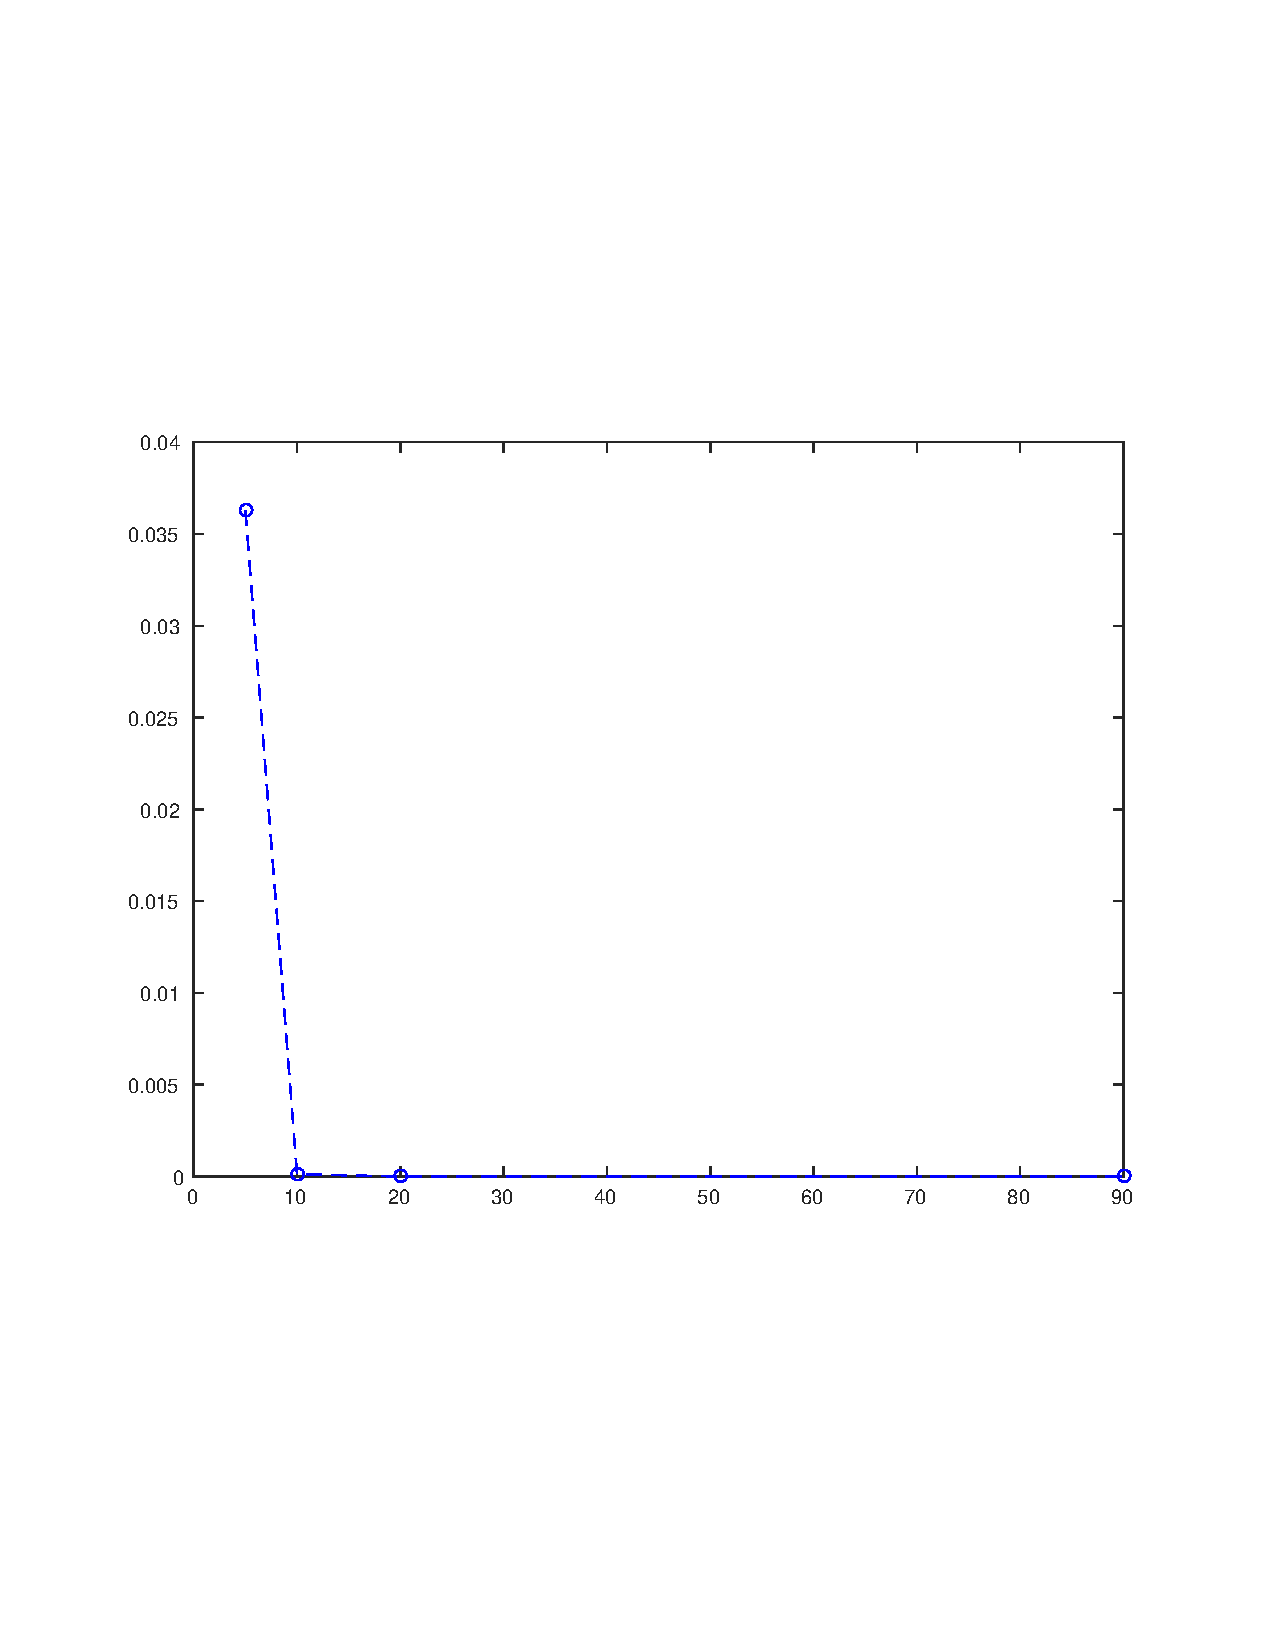
\includegraphics[trim=10mm 70mm 10mm 70mm, width=1.0\textwidth]{../q2_plots}
%\end{figure}
